% --- Bắt đầu nội dung các slide ---

% --- Slide 1: Trang tiêu đề ---
\begin{frame}
    \titlepage
\end{frame}

% --- Slide 2: Thông tin tác giả & người hướng dẫn ---
\begin{frame}
    \centering
    {\Large \textbf{Tác giả:} \TENTACGIA \par}
    {\Large \textbf{Người hướng dẫn:} \TENNGUOIHUONGDAN \par}
    \vspace{0.5cm}
    {\small Khoa: \KHOA \par}
    {\small Trường: \TRUONG \par}
    \vfill
    {\footnotesize \today}
\end{frame}

% ===== SECTION 1: GIỚI THIỆU & BỐI CẢNH =====
\section{Giới thiệu và bối cảnh nghiên cứu}

% --- Slide 3: Vấn đề toàn cầu ---
\begin{frame}{Té ngã: Mối đe dọa toàn cầu}
    \begin{columns}[T]
        \begin{column}{0.48\textwidth}
            \begin{itemize}
                \item Nguyên nhân chính gây chấn thương và tử vong không cố ý.
                \item \textbf{WHO}: $\sim646,000$ ca tử vong/năm; $>80\%$ ở các nước thu nhập trung bình/thấp.
                \item Người cao tuổi: \textbf{30\%} té ngã/năm ở người $>65$ tuổi, tăng lên \textbf{50\%} ở người $>85$ tuổi.
            \end{itemize}
        \end{column}
        \begin{column}{0.48\textwidth}
            \begin{figure}
                \centering
                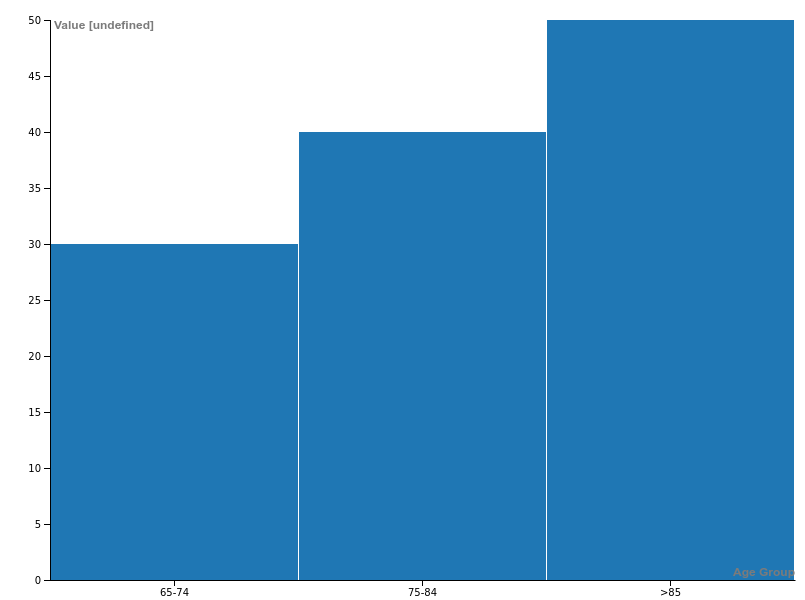
\includegraphics[width=\textwidth]{images/fall_status_who.png}
                \caption{Tỷ lệ té ngã theo nhóm tuổi}
            \end{figure}
        \end{column}
    \end{columns}
\end{frame}

% ===== SECTION 2: TỔNG QUAN VÀ NGHIÊN CỨU LIÊN QUAN =====
\section{Tổng quan và nghiên cứu liên quan}

% --- Slide 4: Tổng quan các phương pháp ---
\begin{frame}{Tổng quan các phương pháp phát hiện té ngã}
    \begin{itemize}
        \item \textbf{Dựa trên thị giác (Vision-based)}: Sử dụng camera và thuật toán nhận diện tư thế người (MediaPipe, OpenPose).
        \item \textbf{Dựa trên cảm biến đeo (Wearable-based)}: Dùng cảm biến quán tính (IMU, MPU6050) trên thiết bị.
        \item \textbf{Kết hợp đa phương thức (Multi-modal)}: Tích hợp dữ liệu từ nhiều nguồn để tăng độ chính xác.
    \end{itemize}
\end{frame}

% --- Slide 5: Nghiên cứu trong và ngoài nước ---
\begin{frame}{Nghiên cứu trong và ngoài nước}
    \begin{columns}[T]
        \begin{column}{0.48\textwidth}
            \textbf{Quốc tế}
            \begin{itemize}
                \item \textbf{Xu hướng}: Sử dụng YOLO, Transformer, AI nhẹ, cảm biến mmWave.
                \item \textbf{Thành tựu}: Giảm false alarm, tối ưu cho thiết bị biên, Sensor Fusion.
            \end{itemize}
        \end{column}
        \begin{column}{0.48\textwidth}
            \textbf{Trong nước}
            \begin{itemize}
                \item \textbf{Thực trạng}: Chủ yếu mô hình thử nghiệm (PoC) với ESP32, Arduino.
                \item \textbf{Hạn chế}: Thiếu dữ liệu lớn, độ chính xác thấp (75-85\%), thiếu tích hợp đa phương thức.
            \end{itemize}
        \end{column}
    \end{columns}
\end{frame}

% ===== SECTION 3: MỤC TIÊU VÀ PHƯƠNG PHÁP NGHIÊN CỨU =====
\section{Mục tiêu và phương pháp nghiên cứu}

% --- Slide 6: Mục tiêu luận văn ---
\begin{frame}{Mục tiêu Luận Văn}
    \begin{itemize}
        \item Xây dựng hệ thống \textbf{giám sát và cảnh báo té ngã} thông minh, \textbf{chi phí thấp}.
        \item Phát hiện \textbf{thời gian thực} (real-time) bằng cách kết hợp dữ liệu cảm biến và hình ảnh.
        \item Thiết kế kiến trúc phân lớp, \textbf{ổn định} và \textbf{dễ mở rộng}.
    \end{itemize}
\end{frame}

% ===== SECTION 4: THIẾT KẾ VÀ THỰC HIỆN HỆ THỐNG =====
\section{Thiết kế và thực hiện hệ thống}

% --- Slide 7: Kiến trúc hệ thống tổng thể ---
\begin{frame}{Kiến trúc hệ thống tổng thể}
    \begin{figure}
        \centering
        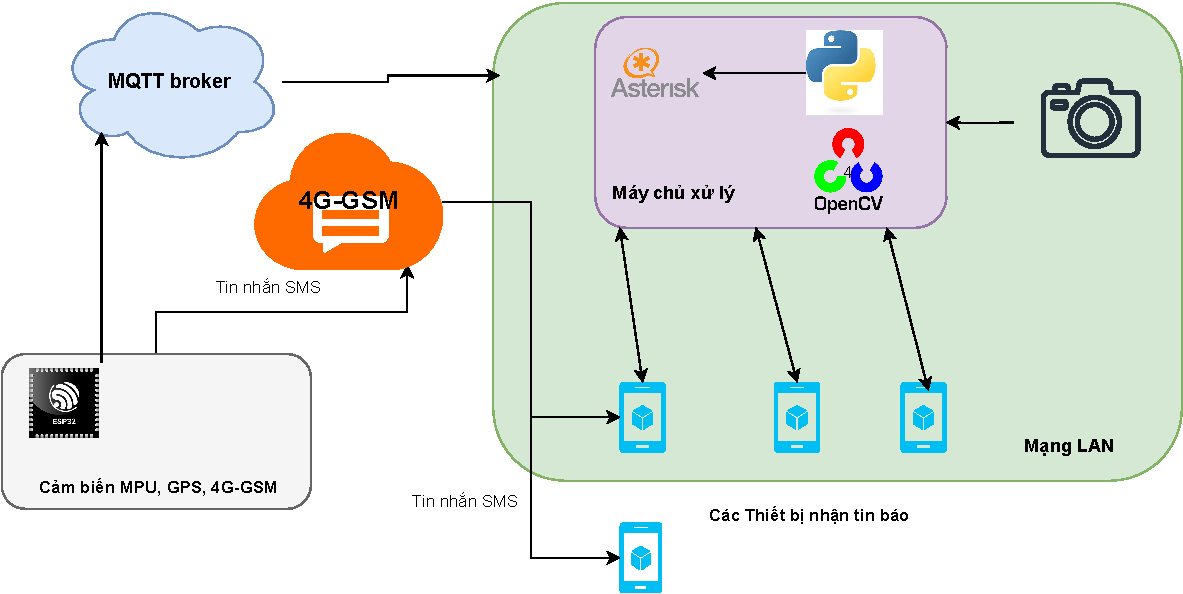
\includegraphics[width=0.8\textwidth]{images/resuilt_structure_diagram.pdf}
        \caption{Sơ đồ hệ thống tổng thể}
    \end{figure}
\end{frame}

% --- Slide 8: Hệ thống nhúng (ESP32) ---
\begin{frame}{Hệ thống nhúng (ESP32)}
    \begin{columns}[T]
        \begin{column}{0.48\textwidth}
            \begin{itemize}
                \item \textbf{Phần cứng}: ESP32, MPU6050, GPS EC800K.
                \item \textbf{Nguyên lý}: Phát hiện té ngã dựa trên ngưỡng động học.
                \item \textbf{Giao tiếp}: Gửi cảnh báo qua \textbf{MQTT và SMS}.
                \item \textbf{Ưu điểm}: Thiết bị độc lập, tiết kiệm năng lượng, dễ mở rộng.
            \end{itemize}
        \end{column}
        \begin{column}{0.48\textwidth}
            \begin{figure}
                \centering
                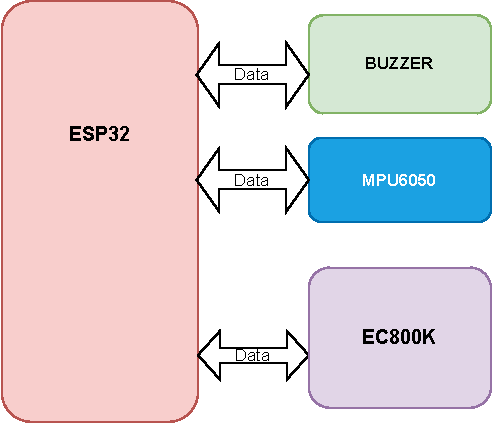
\includegraphics[width=\textwidth]{images/module1_block_diagram-crop.pdf}
                \caption{Sơ đồ nhúng ESP32 \& truyền thông}
            \end{figure}
        \end{column}
    \end{columns}
\end{frame}

% --- Slide 9: Hệ thống phân tích hình ảnh ---
\begin{frame}{Hệ thống phân tích hình ảnh}
    \begin{columns}[T]
        \begin{column}{0.48\textwidth}
            \begin{itemize}
                \item \textbf{Công nghệ}: MediaPipe, OpenCV, YOLO để trích xuất các điểm khớp xương (keypoints) và phân tích tư thế.
                \item \textbf{Quy trình}: Phân tích góc nghiêng, vận tốc, tỉ lệ khung xương để nhận diện té ngã.
                \item \textbf{Thuật toán}: Sử dụng các mô hình học máy (ML) như SVM, Decision Tree.
            \end{itemize}
        \end{column}
        \begin{column}{0.48\textwidth}
            \begin{figure}
                \centering
                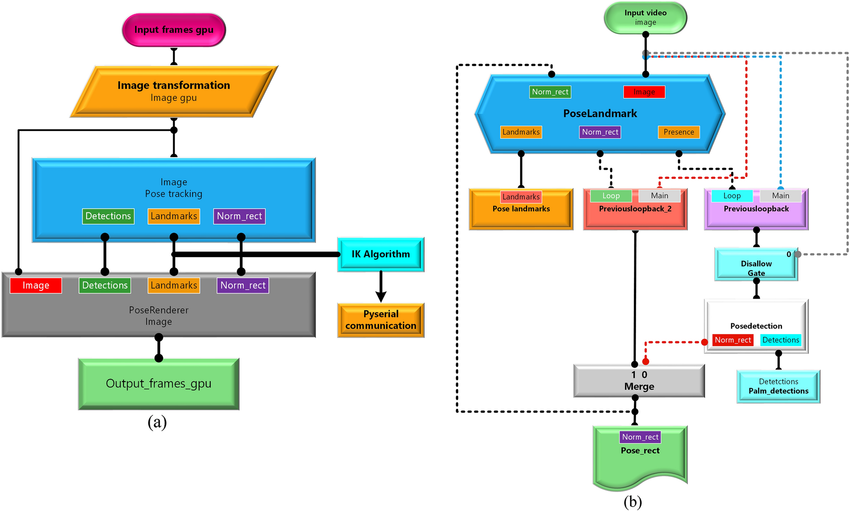
\includegraphics[width=\textwidth]{images/media_pose_pipeline.png}
                \caption{Pipeline MediaPipe + YOLO}
            \end{figure}
        \end{column}
    \end{columns}
\end{frame}

% ===== SECTION 5: KẾT QUẢ VÀ ĐÁNH GIÁ =====
\section{Kết quả và đánh giá}

% --- Slide 10: Hiệu năng và giới hạn ---
\begin{frame}{Hiệu năng và Giới hạn}
    \begin{columns}[T]
        \begin{column}{0.48\textwidth}
            \textbf{Mục tiêu Hiệu năng}
            \begin{itemize}
                \item Tổng độ trễ $<5$ giây.
                \item Độ chính xác $>90\%$, False Alarm $<8\%$.
                \item Uptime dịch vụ MQTT $>99\%$.
            \end{itemize}
        \end{column}
        \begin{column}{0.48\textwidth}
            \textbf{Giới hạn nghiên cứu}
            \begin{itemize}
                \item Hoạt động trong nhà với điều kiện ánh sáng và mạng ổn định.
                \item Nguyên mẫu \textbf{ESP32} chưa tích hợp học sâu toàn phần.
                \item Không phát triển app di động/web phức tạp.
            \end{itemize}
        \end{column}
    \end{columns}
\end{frame}

% --- Kết thúc nội dung các slide ---
